\documentclass{IEEEtran}

\usepackage{tikz}
\usepackage{lipsum}

\usetikzlibrary{shapes.geometric, arrows}

\tikzset{
    objRectangle/.style={rectangle, minimum width=3cm, minimum height=1cm, text centered, draw=black, text width = 5cm},
    objRoundRectangle/.style={rectangle, rounded corners, minimum width=3cm, minimum height=1cm, text centered, draw=black, text width = 5cm},
    arrow/.style={thick, ->, >=stealth}
}

\begin{document}

\lipsum[1]
\begin{figure}[htbp]
    \centering
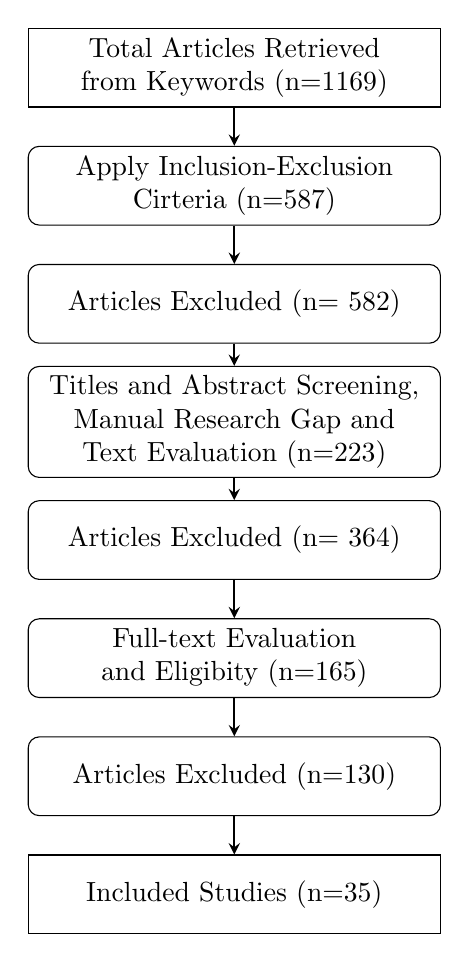
\begin{tikzpicture}[node distance=1.5cm]
    
    \node (001) [objRectangle] {Total Articles Retrieved from Keywords (n=1169)};
    \node (002) [objRoundRectangle, below of=001] {Apply Inclusion-Exclusion Cirteria (n=587)};
    \node (003) [objRoundRectangle, below of=002] {Articles Excluded (n= 582)};
    \node (004) [objRoundRectangle, below of=003] {Titles and Abstract Screening, Manual Research Gap and Text Evaluation (n=223)};
    \node (005) [objRoundRectangle, below of=004] {Articles Excluded (n= 364)};
    \node (006) [objRoundRectangle, below of=005] {Full-text Evaluation and Eligibity (n=165)};
    \node (007) [objRoundRectangle, below of=006] {Articles Excluded (n=130)} ;
    \node (008) [objRectangle, below of=007] {Included Studies (n=35)};
    
    \draw [arrow] (001) -- (002);
    \draw [arrow] (002) -- (003);
    \draw [arrow] (003) -- (004);
    \draw [arrow] (004) -- (005);
    \draw [arrow] (005) -- (006);
    \draw [arrow] (006) -- (007);
    \draw [arrow] (007) -- (008);

\end{tikzpicture}
\caption{Flowchart of the study selection process}
\label{fig:flowchartFilter}
\end{figure}

\lipsum[1]

\end{document}
